\cotefile{62}
\scanpage{20}
% archive sheet number: 19
\mspage{- 20 -}\hfill n$^{\mathrm{o}}$ 276

\handwritten{\S{}}2. - \uline{Anneaux} $\mathrm{m}$-\uline{adiques noethériens}.

Dans tout ce \handwritten{\S{}} on désigne par $A$ un anneau \uline{commutatif noethérien} et par $\mathrm{m}$ un idéal de $A$ ; sauf mention explicite du contraire on munira $A$, et plus généralement tous les $A$-modules considérés, de la topologie $\mathrm{m}$-adique.

1. - \uline{Restriction de la topologie} $\mathrm{m}$-\uline{adique à un sous-module}.

\uline{Théorème} 1 - \uline{Soient} $E$ \uline{un} $A$-\uline{module de type fini et} $F$ \uline{un sous-module de} $E$. \uline{La topologie} $\mathrm{m}$-\uline{adique du} $A$-\uline{module} $F$ \uline{est induite par la topologie} $\mathrm{m}$-\uline{adique de} \unsure{-|} $E$.

Le théorème 1 sera une conséquence du résultat plus précis que voici :

\uline{Lemme d'Artin-Rees} $\handwritten{\unsure{\llcorner|-}}$ \uline{Soient} $A$ \uline{un anneau commutatif noethérien}, $\mathrm{m}$ \uline{un idéal de} $A$, $E$ \uline{un} $A$-\uline{module de type fini et} $F$ \uline{un sous-module de} $E$. \uline{Pour tout entier} $k$ \uline{suffisamment grand on a}
\[
\mathrm{m}^{p}E\handwritten{\cap} F=\mathrm{m}^{p-k}(\mathrm{m}^{k}E\handwritten{\cap} F)\qquad \text{\uline{pour tout}}~p\handwritten{\geqslant} k.
\]

Il suffit évidemment de prouver l'inclusion \unsure{-|}
\[
\mathrm{m}^{p}E\handwritten{\cap} F\handwritten{\subset}\mathrm{m}^{p-k}(\mathrm{m}^{k}E\handwritten{\cap} F)\quad,
\]
puisque l'inclusion opposée est triviale.

Pour cela considérons dans l'anneau de polynômes $A\handwritten{[}X\handwritten{]}$ le sous-anneau $A'$ formé des polynômes $\handwritten{\sum} a_p X^p$ tels que $a_p\handwritten{\in}\mathrm{m}^p$ pour tout $p$. Il est clair qu'en tant qu'algèbre sur $A$, $A'$ est engendré par les $a_i X$ où $a_i$ est un système de générateurs de $\mathrm{m}$ ; par suite $A'$ est un anneau noethérien, par ailleurs gradué.

Formons de même le $A\handwritten{[}X\handwritten{]}$-module
\[
E\handwritten{[}X\handwritten{]}=A\handwritten{[}X\handwritten{]}\underset{A}{\handwritten{\otimes}}E
\]
des polynômes à coefficients dans $E$ ; en tant que $A'$-module, $E\handwritten{[}X\handwritten{]}$ contient le sous-module $E'$ formé des polynomes $\handwritten{\sum} e_p X^p$ tels que $e_p\handwritten{\in}\mathrm{m}^p E$

\scanpage{21}
% archive sheet number: 20
\[
\deleted{(x_1-x_2)(x_3}
\]

\[
\prod_{i\ne j}(x_i-x_j)=\prod_i\left(\frac{f(x_{\deleted{\unsure{j|i}}})}{x_{\deleted{\unsure{j|i}}}-x_i}\right)_{x\to x_i}=\prod_i f'(x_i).
\]
\margin{$(\deleted{x}y+u)^3.+a(y+u)^2$\par $3u+a$\par $u\unsure{:|=} -\frac{a}{3}$}

\[
f(x_i)=
\]

\[
3x^2+2ax+b
\]

\[
(3x_1^2+2ax_1+b)(3x_2^2+2ax_2+b)(3x_3^2+2ax_3+b)
\]

Supposons \uuline{$a=0$} \unsure{on trouve}
\margin{$x_1x_2\quad x_2x_3\quad x_3x_1$\par $x_1x_2\,x_2x_3$}

\[
j=-\frac{27c^2}{\Delta}
\]

\[
\begin{aligned}
\Delta=\prod(3x_{\unsure{1|i}}^2+b)&=27(x_1x_2x_3)^2+9b\bigl(\sum(x_1x_2)^2\bigr)\\
&\qquad+3b^2\sum x_i^2\,\}+b^3\\
&\deleted{=27c^2+9b(b^2-2\sum x_1^2x_2x_3}
\end{aligned}
\]

\[
(x_1x_2x_3)^2=c^2
\]

\[
\sum(x_1x_2)^2=\bigl(\sum x_1x_2\bigr)^2-2\sum x_1^2x_2x_3=
\]

\[
\sum x_i^2x_2x_3=\bigl(\sum x_1^2\bigr)\bigl(\sum x_2x_3
\]

\[
\boxed{\Delta=\deleted{\unsure{9|4}}b^3-27c^2}\;?
\]
\margin{$x_1^{\unsure{3|2}}x_2^2+$}

\[
\prod 3x_i^2+b
\]

\[
\deleted{\bigl(\sum x_{\unsure{1|i}}^2\bigr)^2}
\]

\[
3\sum(x_1x_2)^2+\bigl(\sum x_1x_2\bigr)\bigl(\sum x_i^2\bigr)
\]

\[
\begin{gathered}
\deleted{\unsure{x_1x_2|x_1^2}}\\
\deleted{x_1x_2}
\end{gathered}
\]

\scanpage{22}
% archive sheet number: 21
\mspage{- 9 -}\hfill n$^{\mathrm{o}}$ 276

\uline{Remarque} - La réciproque du corollaire précédent est fausse ; cf. Exerc.N.

4. - \uline{Modules filtrés complets}.

Soit $(E,E_n)$ un module filtré sur un anneau filtré $(A,A_n)$. Puisque la structure uniforme du groupe topologique $E$ est définie par un seul écart, il est clair que $E$ \uline{est complet si et seulement si toute suite de Cauchy, dans} $E$ \uline{est convergente}. Par ailleurs en vertu de l'inégalité
\[
d(x_p,x_q)\handwritten{\leqslant}\underset{p\handwritten{\leqslant} n\handwritten{\leqslant} q-1}{\mathrm{Max}}\;d(x_n,x_{n+1})\quad,
\]
on voit qu'une suite $(x_n)$ de points de $E$ vérifie le critère de Cauchy si et seulement si la suite $d(x_n,x_{n+1})$ tend vers 0, i.e. si et seulement si la suite de terme général $y_n=x_{n+1}-x_n$ tend vers 0 dans $E$. On en déduit :

PROPOSITION 4 - \uline{Pour que le module filtré} $E$ \uline{soit complet}, \uline{il faut et il suffit que toute série d'éléments de} $E$ \uline{dont le terme général tend vers} 0 \uline{soit convergente}.

\uline{Corollaire} 1- \uline{Soit} $(E,E_n)$ \uline{un module filtré complet}. \uline{Tout sous-module fermé de} $E$, \uline{muni de la filtration induite}, \uline{est complet}. \uline{Tout module quotient de} $E$, \uline{muni de la filtration quotient est complet}.
% slanted
\margin{\handwritten{\unsure{faits généraux|fait général}\par \unsure{pour les top|pour les esp.}\par métrisables}}

\margin{\handwritten{!}}L'assertion concernant les sous-modules \uline{résulte} trivialement de la Proposition. D'autre part, si l'on considère, dans un module quotient $E/F$ une série dont le terme général tend vers 0, il est clair que celle-ci est l'image d'une série dans $E$ dont le terme général tend vers 0, donc d'une série convergente dans $E$ ; l'application canonique $E\handwritten{\longrightarrow} E\handwritten{/}F$ étant continue, $E/F$ est complet d'après la proposition 1.

\uline{Corollaire} 2 - \uline{Soient} $(A,A_n)$ \uline{un anneau filtré et complet}, $E$ \uline{un} $A$-\uline{module de type fini}, \uline{filtré par les sous-groupes} $A_n E$. \uline{Alors} $E$ \uline{est complet}

Ecrivons $E=L\handwritten{/}R$ où $L$ est un $A$-module libre de type fini ; la filtration de $E$ par les $A_n E$ se déduit alors de la filtration analogue de $L$ ;

\scanpage{23}
% archive sheet number: 22
\[
\frac{(t+1)(2t-1)(t-2)}{t(t-1)}
=\unsure{-|=|}\frac{(2x_1\unsure{-|+}x_2-x_3)(2x_2-x_3-x_1)(2x_3-x_1-x_2)}
{(x_1-x_2)(x_2-x_3)(x_3-x_1)}.
\]

\[
\deleted{x_1x_2x_3}\quad
\boxed{j=-\frac{1}{27\Delta}\bigl[(2x_1-x_2-x_3)(2x_2-x_3-x_1)(2x_3-x_1-x_2)\bigr]^2}.
\]

\margin{$\sum x_1=-a$\par $\sum x_1x_2=b$\par $x_1x_2x_3=-c$}
\[
\Delta=\bigl((x_1-x_2)(x_2-x_3)(x_3-x_1)\bigr)^2
\]

\[
j=\frac{\bigl[(3x_1+a)(3x_2+a)(3x_3+a)\bigr]^2}{-27\Delta}
\]

\[
\deleted{\frac{27}{-\Delta}\bigl[(a/3+x_1)(a/3+x_2)(a/3+x_3)\bigr]^2}
\]

\[
\deleted{(a/3)}
\]

\[
\begin{aligned}
\sqrt{-27\Delta j}&=a^3+3a^{\unsure{2|3}}(\deleted{\unsure{-|}}x_1+x_2+x_3)+\deleted{\unsure{2|3}}9a(x_1x_2+x_2x_3+x_3x_1)\\
&\qquad+27\deleted{\unsure{a|b}}x_1x_2x_3\\
&=a^3-3a^3+9\unsure{b|ab}-27\deleted{\unsure{a|b}}c\\
&=-2a^3+9ab-27c
\end{aligned}
\]

\[
\boxed{j=\frac{(27c+2a^3-9ab)^2}{-27\Delta}}
\]

\[
\deleted{\prod(x_1^2+x_2^2-2x_1x_2)=}
\]

\scanpage{24}
% archive sheet number: 23
\mspage{- 10 -}\hfill n$^{\mathrm{o}}$ 276

en vertu du corollaire précédent on peut donc se ramener\handwritten{/}au cas où $E$ est \uline{libre}, i.e. est produit direct d'un nombre fini de facteurs isomorphes à $A$. Raisonnant par récurrence, on est alors ramené à établir que si deux modules $E$ et $F$ (munis des filtrations associées à la filtration de $A$) sont complets il en est de même du module $E\times F$ : or les relations
\[
A_p E\times A_q F\handwritten{\subset} A_n(E\times F)\handwritten{\subset} A_n E\times A_n F\qquad(p,q\handwritten{\leqslant} n)
\]
montrent que $E\times F$ est le produit direct des groupes \uline{topologiques} $E$ et $F$. il est donc complet si $E$ et $F$ le sont.

PROPOSITION 5 - \uline{Soient} $A$\uline{un anneau commutatif}, $\mathrm{m}$ \uline{un idéal de} $A$, \uline{et supposons l'anneau} $A$ \uline{séparé} (resp. complet) \uline{pour la topologie} $\mathrm{m}$-\uline{adique}. \uline{Alors L'anneau de séries formelles} $A\handwritten{[[}X\handwritten{]]}$, \uline{filtré par les puissances de l'idéal} \inserted{\handwritten{engendré}} \uline{par} $\mathrm{m}$ \uline{et} $X$, \uline{est séparé} (resp. \uline{complet}).
% slanted
\margin{\handwritten{Dire \unsure{que la|que} \unsure{top. en quest.|top. en question|topologie} celle de la conv. simple des coefficients.}}

Soit $\mathrm{n}$ l'idéal de $B={}'A\handwritten{[[}X\handwritten{]]}$ engendré par $\mathrm{m}$ et $X$ : c'est l'ensemble des séries formelles $\handwritten{\sum} a_n X^n$ telles que $a_0\handwritten{\in}\mathrm{m}$. On déduit de là que pour tout entier $p$, l'idéal $\mathrm{n}^p$ est formé des séries $\handwritten{\sum} a_n X^n$ telles que l'on ait $a_n\handwritten{\in}\mathrm{m}^{p-n}$ pour $0\handwritten{\leqslant} n\handwritten{\leqslant} p$. Il résulte immédiatement de là que $B$ est séparé si $A$ est séparé. Supposons de plus $A$ complet, et considérons dans $B$ une série $\handwritten{\sum} y_i$ dont le terme général
\[
y_i=\handwritten{\sum} a_{in}X^n
\]
tend vers 0 ; pour tout entier $p$ on a donc
\begingroup\makeatletter\tagsleft@true\makeatother
\[
a_{in}\handwritten{\in}\mathrm{m}^{p-n}\qquad(0\handwritten{\leqslant} n\handwritten{\leqslant} p)\ \text{pour }i>i_p.\tag*{(1)}
\]
\endgroup

En fixant $n$ et en faisant varier $p$ on voit, puisque $A$ est complet, que la série $\handwritten{\sum}_i a_{in}$ \unsure{c\deleted{n}onverge|converge} dans $A$ ; soit $a_n$ l'une des ses sommes (on ne suppose pas $A$ séparé). En vertu de (1) et du fait que les puissances de $\mathrm{m}$ sont fermées dans $A$, on a, quels que soient $n$ et $p\handwritten{\geqslant} n$, la relation
\[
\handwritten{\sum}_{i>i_p}\unsure{a|e}_{in}\handwritten{\in}\mathrm{m}^{p-n}
\]

\scanpage{25}
% archive sheet number: 24
\[
y^2=4x^3-h(x+1)\qquad h=27j(j-2^6.3^3)^{-1}
\]

\[
\deleted{y^2=\deleted{\unsure{a|4}}x^3\unsure{+|-}bx^2+cx+d}
\qquad y^2=x^3+\underset{1}{\unsure{a|g}}x^2+\underset{2}{b}x+\underset{3}{c}
\]

\diagram{\begin{tikzcd}[ampersand replacement=\&,column sep=small,row sep=small]
x_1\arrow[d]\&\unsure{.|}x_2\arrow[d]\&x_3\arrow[d]\&\deleted{\infty}x_4\arrow[d]\\
\infty\&0\&1\&t
\end{tikzcd}}

\diagram{\begin{tikzcd}[ampersand replacement=\&,column sep=small]
\infty\arrow[rrr,dash,start anchor=north,end anchor=north,to path={-- ++(0,.30) -| (\tikztotarget)}]\arrow[rr,dash,start anchor=south,end anchor=south,to path={-- ++(0,-.23) -| (\tikztotarget)}]
\&0\arrow[rr,dash,start anchor=north,end anchor=north,to path={-- ++(0,.18) -| (\tikztotarget)}]\arrow[r,dash,start anchor=south,end anchor=south,to path={-- ++(0,-.14) -| (\tikztotarget)}]\&1\&t
\end{tikzcd}}

\diagram{\begin{tikzcd}[ampersand replacement=\&,column sep=0pt]
((\&0,\arrow[rrr,dash,start anchor=south,end anchor=south,to path={-- ++(0,-.16) -| (\tikztotarget)}]\&1,\arrow[rr,dash,start anchor=south,end anchor=south,to path={-- ++(0,-.16) -| (\tikztotarget)}]\&\infty,\&t\&))=((x_{\unsure{2|1}},x_3\,x_1,x_4))
\end{tikzcd}}

\[
\begin{aligned}
\frac{x_1-x_3}{x_1-x_4}:\frac{x_2-x_3}{x_2-x_4}&=\frac{0-\infty}{0-t}:\frac{1-\infty}{1-t}\\
&=\frac{1-t}{-t}=-\frac{1}{t}+1
\end{aligned}
\]

\[
\frac{t-1}{t}\qquad\frac{t-\infty}{t-0}:\frac{\unsure{1|t}-\infty}{1-0}
\]

\[
\deleted{\unsure{t|\frac{1}{t}|4}}
\]

\[
t=\frac{1-\infty}{1-0}:\frac{t-\infty}{t-0}=\frac{x_3-x_1}{x_3-x_2}:\frac{x_4-x_1}{x_4-x_2}
\]

Si $x_4=\infty$, \unsure{on trouve}

\[
\boxed{t=\frac{x_3-x_1}{x_3-x_2}}\qquad t-1=\frac{x_2-x_1}{x_3-x_2}
\]
\margin{$\frac{c-a}{c-b}\ \big|\ \frac{c-b}{c-a}$\par $\left.\overline{\frac{a-b}{a-c}}\right|\quad \frac{a-b}{c-b}\unsure{=|-|\cdot}\frac{b-a}{b-c}$}

\[
\begin{aligned}
t+1&=\frac{2x_3-x_1-x_2}{x_3-x_2}\\
2t-1&=\frac{x_3-2x_1+x_2}{x_3-x_2}\\
t-2&=\frac{-x_3\unsure{\dot{-}|-}x_1+2x_2}{x_3-x_2}
\end{aligned}
\]

\scanpage{26}
% archive sheet number: 25
\mspage{- 11 -}\hfill n$^{\mathrm{o}}$ 276

\figure{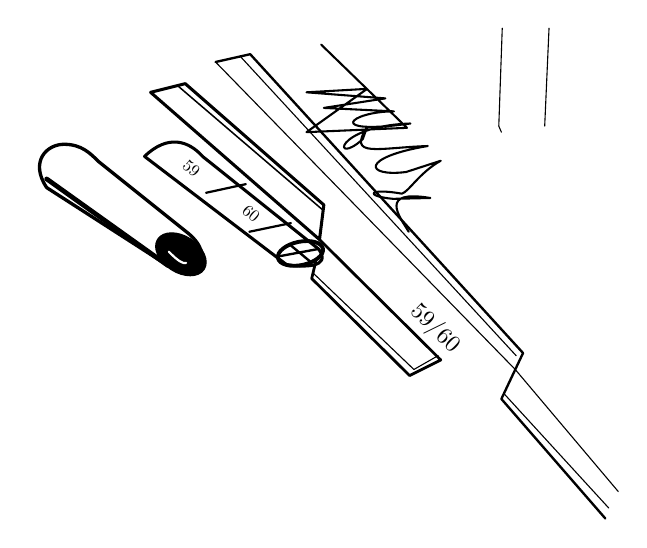
\begin{tikzpicture}[x=.11cm,y=.11cm,line cap=round,line join=round]
\draw[line width=1.2pt] (0,30) .. controls (-2,33) and (0,35) .. (2,35) .. controls (4,35) and (5,34) .. (6,33) -- (16,25) .. controls (20,22) and (17,19) .. (14,21) -- cycle;
\draw[line width=1.7pt] (0,31) -- (14,21);
\filldraw[rotate around={-33:(15.5,22.3)}] (15.5,22.3) ellipse (3.2 and 2.1);
\draw[white,line width=.8pt] (14.1,22.6) .. controls (15.2,21.5) and (15.7,21.2) .. (16.1,21.3);
\draw[line width=1.1pt] (12,41) -- (16,42) -- (32,28) -- (31.5,24) -- cycle;
\draw[line width=.55pt] (15.2,41.7) -- (31.9,27.4);
\draw[line width=1.1pt] (11.3,33.6) .. controls (14,36.2) and (16.4,35.4) .. (18,33.6) -- (31.4,22.9) .. controls (33,20.7) and (29.5,20.8) .. (27.7,21.1) -- cycle;
\draw[line width=.8pt] (18.4,29.4) -- (23,30.4) (23.4,24.9) -- (28.2,25.9);
\node[rotate=-40,scale=.61] at (16.7,32.2) {\handwritten{59}};
\node[rotate=-40,scale=.61] at (23.6,27.0) {\handwritten{60}};
\draw[line width=1.4pt,rotate around={12:(29.3,22.4)}] (29.3,22.4) ellipse (2.65 and 1.35);
\draw[line width=.85pt] (27,22.1) -- (31.3,22.9) (28.1,23.4) -- (30.5,21.4);
\draw[line width=1pt] (31.5,24) -- (45.5,10.1) -- (41.9,8.3) -- (30.6,19.5) -- (31.1,21.6);
\draw (30.8,20.1) -- (42.4,9.0) -- (45.2,10.6);
\draw[line width=.85pt] (19.5,44.5) -- (23.5,45.4) -- (55.0,10.9) -- (52.5,5.6) -- (64.5,-8.2);
\draw (22.4,45.1) -- (54.2,10.6) (19.5,44.5) -- (54.1,9.0) -- (66,-5.1) (52.9,6.1) -- (64.9,-7);
\node[rotate=-44,scale=.85] at (44.8,13.7) {\handwritten{59/60}};
\draw[line width=.75pt] (31.7,46.5) -- (41.6,36.9) -- (30,36.4) -- (37,41.4) -- (30,41) -- (39.1,40.3) -- (32,39.2) -- (40.1,38.8) .. controls (35,38.8) and (32,36) .. (42,37.4) .. controls (33,37.1) and (33,32.4) .. (36.5,35.6) -- (37,37) .. controls (34.7,33.4) and (38.2,34.6) .. (44,34.8) .. controls (36.2,33.5) and (36.7,31.2) .. (41.5,31.8) -- (45.5,33.1) .. controls (43,31.7) and (41.8,29.5) .. (41,29.3) .. controls (37,30) and (36.7,29.0) .. (40,28.7) -- (44.3,28.8) .. controls (38.3,29.8) and (40.7,26.7) .. (41.8,24.9);
\draw[thin] (52.6,48.4) -- (52.2,37.1) -- (52.5,36.4) (58,48.4) -- (57.5,37.1);
\end{tikzpicture}}

et par conséquent :
\[
a_n-\handwritten{\sum}_{i=\unsure{o|0}}^{i=i_p}a_{in}\handwritten{\in}\handwritten{\unsure{\mathfrak{m}|\mathrm{m}}}^{p-n}\quad.
\]

Considérant alors la série formelle $y=\handwritten{\sum} a_n X^n$, la relation précédente montre que l'on a
\[
y-\handwritten{\sum}_{i=o}^{i=i_p}y_i\handwritten{\in}\handwritten{\unsure{\mathfrak{n}|\mathrm{n}}}^p
\]
ce qui prouve que la série $\handwritten{\sum} y_i$ converge vers $y$, d'où la proposition.

\uline{Corollaire} - \uline{Soit} $A$ \uline{un anneau commutatif},. \uline{L'anneau de séries formelles} $A\handwritten{[[}X_1,\ldots,X_r\handwritten{]]}$ \uline{filtré par les puissances de l'idéal} $(X_1,\ldots X_r)$, \uline{est séparé et complet}.

5. - \uline{Modules de type fini sur un anneau filtré complet}.

Soient $(E,E_n)$ et $(F,F_n)$ deux modules filtrés sur un anneau filtré $(A,A_n)$ par un \uline{homomorphisme} $u:(E,E_n)\handwritten{\longrightarrow}(F,F_n)$ on entendra tout homomorphisme $u:E\handwritten{\longrightarrow} F$ de $A$-modules, tel que l'on ait
\[
u(E_n)\handwritten{\subset} F_n
\]
pour tout $n$. Si les filtrations de $E$ et $F$ sont associées à la filtration donnée de $A$, tout homomorph\deleted{\unsure{s|i}}isme de $A$-modules est un homomorphisme de modules filtrés\unsure{,|.}

Il est clair que tout homomorphisme $u:(E,E_n)\handwritten{\longrightarrow}(F,F_n)$ définit canoniquement un homomorphisme $G(u):G(E)\handwritten{\longrightarrow} G(F)$ des $G(A)$-modules gradués associés, obtenu par passage au quotient.

PROPOSITION 6 - \uline{Soient} $(E,E_n)$ \uline{et} $(F,F_n)$ \uline{deux modules filtrés sur un anneau filtré}, \uline{et} $u:(E,E_n)\handwritten{\longrightarrow}(F,F_n)$ \uline{un homomorphisme de modules filtrés}. \uline{Supposons remplies les conditions suivantes} :

a) : $(E,E_n)$ \uline{est complet}.

b) : $(F,F_n)$ \uline{est séparé}.

c) : \uline{l'homomorphisme associé} $G(u)$ \uline{est surjectif}\unsure{,|.}

\scanpage{28}
% archive sheet number: 27
$P^1_S$ sections $0,1,\infty$. Le groupe des automorphismes s'identifie au groupe $\unsure{\mathfrak{S}|\mathfrak{G}}_3$ des permutations des trois objets $0,1,\infty$, groupe \unsure{à|:} 6 éléments $1,\varphi,\psi,\lambda,\mu,\nu$

\begingroup\makeatletter\tagsleft@true\makeatother
\[
\left\{\begin{aligned}
\varphi(t)&=1-\frac1t\\
\psi(t)&=\frac1{1-t}
\end{aligned}\right.\qquad
\text{2 permutations circulaires non triviales sur }0,1,\infty
\tag*{(1)}
\]
\endgroup

\begingroup\makeatletter\tagsleft@true\makeatother
\[
\left\{\begin{array}{ll||l}
\lambda t=\frac1t&\text{transposition de }0,\infty&1\\
\mu t=1-t&\text{transposition de }0,1&\infty\\
\nu t=1+\frac1{t-1}=\frac{t}{t-1}&\text{transposition de }1,\infty&0
\end{array}\right.
\tag*{(2)}
\]
\endgroup
% slanted
\margin{\unsure{renommer|renumérer|prenons|pour mémoire|pour moi} :\par $\left\{\begin{aligned}\lambda t&=1-\unsure{t|1}\\ \mu t&=\tfrac{t}{t-1}\\ \nu t&=1/t\end{aligned}\right.$\par ??}

\begingroup\makeatletter\tagsleft@true\makeatother
\[
\boxed{\begin{aligned}\varphi^2&=\psi\qquad\psi^2=\varphi\\
\deleted{\unsure{\psi\varphi|\varphi\psi}}\quad\varphi\psi&=\psi\varphi=1\end{aligned}}
\tag*{3 a)}
\]
\endgroup

\begingroup\makeatletter\tagsleft@true\makeatother
\[
\boxed{\lambda^2=\mu^2=\nu^2=1}\tag*{b)}
\]
\endgroup

\begingroup\makeatletter\tagsleft@true\makeatother
\[
\boxed{\begin{aligned}\lambda\mu&=\mu\nu=\nu\lambda=\varphi\\
\mu\lambda&=\nu\mu=\lambda\nu=\psi\end{aligned}}\tag*{c)}
\]
\endgroup

\begingroup\makeatletter\tagsleft@true\makeatother
\[
\boxed{\begin{array}{l|l}
\varphi\lambda=\mu\varphi=\nu&\psi\nu=\mu\psi=\lambda\\
\varphi\mu=\nu\varphi=\lambda&\psi\mu=\lambda\psi=\nu\\
\varphi\nu=\lambda\varphi=\mu&\psi\lambda=\nu\psi=\mu
\end{array}}\tag*{d)}
\]
\endgroup

$1,\varphi,\psi$ groupe cyclique d'ordre 3, de \unsure{générateurs|engendré par} $\varphi$ et $\psi$, invariant dans $\mathfrak{S}_3$

Le quotient est $\mathbb{Z}/2$ et $\mathfrak{S}_3$ est produit semi-direct ; il y a trois sous-groupes \unsure{sections|section}, engendrés resp\textsuperscript{t}. par $\lambda,\mu,\nu$ (les seuls \unsure{éléments} d'ordre 2)

\begingroup\makeatletter\tagsleft@true\makeatother
\[
\left\{\begin{aligned}
{}^\varphi\lambda&=\mu&{}^\varphi\mu&=\nu.&{}^\varphi\nu&=\lambda\\
{}^\psi\nu&=\mu&{}^\psi\mu&=\lambda&{}^{\psi}\lambda&=\nu
\end{aligned}\right.\tag*{4)}
\]
\endgroup

\begingroup\makeatletter\tagsleft@true\makeatother
\[
\left\{\begin{aligned}
{}^\lambda\varphi&={}^\mu\varphi={}^\nu\varphi=\psi\\
{}^\lambda\psi&={}^\mu\psi={}^\nu\psi=\varphi
\end{aligned}\right.\tag*{5)}
\]
\endgroup

De plus, on a dans $P^1$ un automorphisme $\unsure{\sigma|5}$ \deleted{\unsure{de|dans}} de carré 1, donné par
\begingroup\makeatletter\tagsleft@true\makeatother
\[
\sigma t=\frac{t-2}{2t-1}\qquad[\sigma^2=\mathrm{id}]\tag*{6)}
\]
\endgroup
\unsure{permutant :|permutant à|permutable à|Normalisateur :} $\mathfrak{S}_{6}$ (c'est d'ailleurs le seul, sauf

\scanpage{29}
% archive sheet number: 28
\mspage{-39-}\hfill n$^{\mathrm{o}}$ 272

Corollaire 1.- \uline{Pour toute famille} $a_i\handwritten{\in} A_i$ $(1\handwritten{\leqslant}i\handwritten{\leqslant}n)$, \uline{il existe} $x\handwritten{\in}B$ \uline{tel que} $x\handwritten{\equiv}a_i\,(\mathrm{mod.}\ \underline{p}_i)$.

Puisque les $\underline{p}_i$ sont des idéaux maximaux de $B$, on a $B_{\underline{p}_i}\handwritten{/}\underline{p}_i B_{\underline{p}_i}=B\handwritten{/}\underline{p}_i$, et l'on peut donc supposer que $a_i\handwritten{\in}B$ pour tout $i$. Dans ce cas, le corollaire signifie que l'application $B\handwritten{\to}\handwritten{\prod} B\handwritten{/}\underline{p}_i$ est surjective, ce qui est un résultat bien connu (cf.Ch.I, \handwritten{\S}2, cor. à la prop.4).

Corollaire 2.- \uline{Il existe des éléments} $x_i\handwritten{\in}K$ \uline{tels que} $v_i(x_i)=0$ \uline{et} $v_j(x_i)\handwritten{>}0$ \uline{pour} $i\handwritten{\ne}j$.

Pour chaque indice $i$, on applique le cor.1 à la famille $a_j=0$ si $j\handwritten{\ne}i$, $a_i=1$.

Corollaire 3.- \uline{Tout anneau de valuation contenant} $B$ \uline{contient l'un des} $A_i$.

Soit $A$ un anneau de valuation contenant $B$, et soit $\underline{p}=\underline{m}(A)\handwritten{\cap}B$; il existe un idéal maximal $\underline{p}_i$ de $B$ contenant $\underline{p}$, d'ou $A_i=B_{\underline{p}_i}\handwritten{\unsure{<|\subset}}B_{\underline p}\handwritten{\subset}A$. \handwritten{[}En fait, on a $A=B_{\underline p}$ en vertu de la prop.1\unsure{;|,} mais on s'en fout.\handwritten{]}

2. \uline{Valuations indépendantes}.

Définition 1.- \uline{Soient} $A$ \uline{et} $A'$ \uline{deux anneaux de valuation d'un même corps} $K$. \uline{On dit que} $A$ \uline{et} $A'$ \uline{sont indépendants s'il n'existe aucun sous-anneau de} $K$, \uline{distinct de} $K$, \uline{les contenant}.

Bien entendu, on dit que deux valuations $v$ et $v'$ de $K$ sont \uline{indépendantes} si leurs anneaux sont indépendants.

\uline{Exemple}. Si $A$ et $A'$ sont \uline{distincts} et sont tous deux des anneaux de valuation de \uline{rang} 1, ils sont indépendants, en vertu de la prop.7 du \handwritten{\S}4.

Proposition 3.- (\uline{théorème d'approximation}). \uline{Soient} $v_i$ $(1\handwritten{\leqslant}i\handwritten{\leqslant}n)$ \uline{des valuations deux à deux indépendantes d'un corps} $K$, \uline{et soient} $\handwritten{\Gamma}_i$ \uline{leurs groupes des ordres}. \uline{Soient} $a_i\handwritten{\in}K$ \uline{et} $\handwritten{\gamma}_i\handwritten{\in}\handwritten{\Gamma}_i$ $(1\handwritten{\leqslant}i\handwritten{\leqslant}n)$. \uline{Il existe alors} $x\handwritten{\in}K$ \uline{tel que} $v_i(x-a_i)\handwritten{\geqslant}\handwritten{\gamma}_i$ \uline{pour tout} $i$.

\scanpage{30}
% archive sheet number: 29
l'identité). Il transforme $0,1,\infty$ en
\begingroup\makeatletter\tagsleft@true\makeatother
\[
\left\{\begin{aligned}
\sigma0&=2\\
\sigma1&=-1\\
\sigma\infty\unsure{.|}&=\tfrac12
\end{aligned}\right.\tag*{7)}
\]
\endgroup
% slanted
\margin{\unsure{Prouver|Préciser} : le normalisateur de $\unsure{\mathfrak{S}|\mathfrak{G}}_3$ dans $\mathrm{Aut}_S P^1_S$ est $\mathfrak{S}_3\times(\deleted{\unsure{\mathfrak{S}|\sigma}}\mathbb{Z}/2)$}

La \unsure{différente|différent} de $\mathfrak{S}_3$ -- ens des pts de ramification -- est formé des ens. des pts où un des cinq \unsure{opérateurs} $\lambda\mu\nu\varphi\psi$ est de l'inertie.

Pour $\lambda,\mu,\nu$ on trouve les sections $(\deleted{\unsure{0|t}}1,\deleted{\unsure{2|1}}-1)$ $(\infty,1/2)$ $(0,2)$, [\unsure{stable|stables} par $\unsure{S|\sigma}$]. Pour $\varphi$ (et $\psi$, c'est pareil), on trouve $1-\frac1t=t$ ou
\begingroup\makeatletter\tagsleft@true\makeatother
\[
t^2-t+1=0\tag*{8)}
\]
\endgroup
i.e. l'équation cyclotomique $\boxed{\Phi_6(t)=0}$. \deleted{\unsure{la|le|6}}

\deleted{\unsure{définit aussi|définit ainsi|définit un|déduit aussi}} C'est aussi l'ens $\overline{S}$ des pts fixes sous $\sigma$.

[Il est non ramifié \inserted{sur $S$} aux pts $s\in S$ tels que $k(s)$ soit de car. $\ne2,3$.]. $\mathbb{Z}_2=\mathfrak{S}_3/(\mathbb{Z}/3)$ y\unsure{:|} opère, de façon \uline{non triviale} aux pts où il est non ramifié sur $S$.

\margin{\unsure{Ceci suppose|bien supposer|en supposant|les pts} qu'il n'y a pas de car. 2 ou 3 dans $S$}D'autre part, le \unsure{schém.|schéma} \inserted{$G$} des automorphismes de $P^1$ qui laissent $\overline{S}$ \unsure{globalement} invariant est une extension de $\mathbb{Z}_2$ [automorphismes de $\overline{S}$] par $(G_m)_S$ \uline{tordu} ---- [par le rev. cyclotomique]

\scanpage{31}
% archive sheet number: 30
\mspage{- 47 -}\hfill n$^{\mathrm{o}}$ 272

$n=\handwritten{[}L:K\handwritten{]}$. \quad b) \uline{L'intersection} $B$ \uline{des} $A_i$ \uline{est la cl\handwritten{\^}{o}ture intégrale de} $A$ dans $L$.

c) \uline{Si l'on pose} $\underline{p}_i=B\handwritten{\cap}\underline{m}(A_i)$, \uline{les idéaux} $\underline{p}_i$ \uline{sont des idéaux maximaux de} $B$, \uline{distincts} : \uline{tout idéal maximal de} $B$ \uline{est égal à l'un des} $\underline{p}_i$ \uline{et l'on a} \unsure{.|} $A_i=B_{\underline{p}_i}$.

Nous noterons $v_i$ (resp.$v$) des valuations associées aux $A_i$ (resp. à $A$), et $\Gamma_i$ (\unsure{r\.esp.|rèsp.|resp.}$\Gamma$) les groupes des ordres correspondants. Le groupe $\Gamma$ s'identifie à un sous-groupe de chacun des groupes $\Gamma_i$.

Montrons d'abord que l'on ne peut pas avoir $A_i\handwritten{\supset}A_j$ si $i\handwritten{\not}=j$. En effet, d'après ce que l'on a vu au \handwritten{\S}4, le groupe $\Gamma_i$ s'identifierait à un groupe quotient $\Gamma_j\handwritten{/}H$, où $H$ est un sous-groupe isolé de $\Gamma_j$ ; puisque l'application canonique $\Gamma\handwritten{\longrightarrow}\Gamma_j\handwritten{\longrightarrow}\Gamma_j\handwritten{/}H=\Gamma_i$ est une injection, on a $\handwritten{\Gamma\cap}H=\handwritten{\{}0\handwritten{\}}$ dans $\Gamma_j$, ce qui\unsure{.|...|} montre que $H$ est isomorphe à un sous-groupe de $\Gamma_j\handwritten{/}\Gamma$ ; comme ce dernier groupe est fini (prop.1), on a $H=0$, et les valuations $v_i$ et $v_j$ sont équivalentes, d'où $A_i=A_j$ contrairement à l'hypothèse $i\handwritten{\not}=j$.

Montrons maintenant que le nombre des $A_i$ est \unsure{1|,|'} $\handwritten{\leqslant}n$. Supposons donc qu'il existe $s$ anneaux $A_i$ distincts, avec $s\handwritten{>}n$. D'après le cor. 2 à la \unsure{.|}prop.2 du \handwritten{\S}6, (qui est applicable, en vertu de ce que l'on vient de voir), il existe des éléments $x_i\handwritten{\in}L$, $1\handwritten{\leqslant}i\handwritten{\leqslant}s$, tels que $v_i(x_i)=0$ et $v_j(x_i)\handwritten{>}0$ pour $i\handwritten{\not}=j$. Montrons que les $x_i$ sont linéairement indépendants sur $K$, ce qui fournira la contradiction cherchée. Supposons que l'on ait une relation linéaire non triviale :
\[
\handwritten{\sum} a_i x_i=0\quad,\ \text{avec }a_i\handwritten{\in}K.
\]

Soit $a_j$ celui des $\unsure{a'_i|a_i}$ dont la valuation est minimum ; quitte à multiplier les $a_i$ par $a_j^{-1}$ on peut supposer que $a_j=1$. On a alors une relation :

\scanpage{32}
% archive sheet number: 31
\diagram{\begin{tikzcd}[ampersand replacement=\&]
e \arrow[r] \& G_m^{\text{tordu}} \arrow[r] \& G \arrow[r] \& Z/2 \arrow[r] \& e\\
e \arrow[r] \& \mathbb Z/3 \arrow[u]\arrow[r] \& \mathfrak{S}_3 \arrow[r] \& \mathbb Z/2 \arrow[u,equal]\arrow[r] \& e
\end{tikzcd}}

On suppose tjrs qu'il n'y a pas de \unsure{pt|pts} $s$ de car. 2 ou 3 dans $S$. Alors \deleted{\unsure{$\mathfrak S_3$|$G$|le} \unsure{opère|groupe}} $\mathfrak S_3\times Z_2$ opère ``tamely'' sur $P^1_S$ [en effet, il est compatible avec la fibration $P^1_S\to S$, et opère\unsure{'|} ``tamely'' sur les fibres $\ldots$] Le quotient \inserted{par \unsure{ce|un|le} groupe ou un ss-groupe} \deleted{s'identifie} \inserted{est isomorphe} encore à $P^1_S$ [car il est \uline{\unsure{lisse|simple}} sur $S$, et rationnel sur $S$ d'après Lüroth]. Les schémas de pts fixes $(0,1,\infty)$ $(\unsure{2|3},-1,1/2)$ $(\bar S=x',x'')$ -- qui sont disjoints, et chacun stables sous $\mathfrak S_3$, qui \deleted{y} \inserted{sur chacun} opère de façon \deleted{\unsure{simplement}} transitive sur chaque fibre; donc on obtient dans $P^1_S/\mathfrak S_3$ trois \uline{sections} distinctes [à expliciter $\ldots$] qu'on peut utiliser pour identifier $P^1_S/\mathfrak S_{\unsure{3|2}}$ \unsure{.|à} $P^1_S$ avec les sections $\infty,0,1$. De $=$, \deleted{de se donner des \unsure{sect.|sect}} $P^1_S/(\mathbb Z/3)$ est muni d'abord de deux sections qui correspondent à $(0,1,\infty)$ et $(2,-1,1/2)$, et qui

\scanpage{33}
% archive sheet number: 32
\mspage{- 46 -} \hfill n° 272

l'application identique $k\handwritten{\to} k$, on a $\Omega\handwritten{\not}=\varnothing$. Soit $(F,\psi)$ un élément maximal de $\Omega$. Montrons d'abord que $L$ est \uline{algébrique} sur $F$ ; sinon, en effet, il existerait $X\in L$ transcendant sur $F$, et $L$ contiendrait $F'=F(X)$ ; en composant la place $\lambda:F(X)\handwritten{\to} F$ donné par $f\handwritten{\to} f(0)$ avec la place $\psi:F\handwritten{\to} k$, on obtiendrait une place de $F'$ qui serait l'identité sur $k$, contrairement au caractère maximal de $(F,\psi)$. Donc $L\handwritten{/}F$ est algébrique. Soit Alors $\psi'$ une place de $L$ à valeurs dans une extension $k'$ de $k$ qui prolonge $\psi$ ; une telle extension existe d'après la prop.4 du § 2 ; en vertu de la prop.3 , ci-dessus\unsure{,|;} $\psi'(L)$ est algébrique sur $\psi(F)=k$, donc $\psi'(L)=k$, pui sque $k$ est algébriquement clos, et la place $\psi'$ est la place cherchée.

\handwritten{[}Ce n° pourrait remonter bien plus tôt à condition de donner une démonstration directe de la prop.3, ce qui n'est pas bien difficile. Est-ce que cela en vaut la peine ? La prop.4 est un résidu des rédactions antérieures (où elle était démontrée en même temps que le th. d'extension des valuations) ; le rédacteur ne pense pas qu'elle ait jamaix servi à quoi que ce soit, et ne l'a gardée que sur les instances de Samuel ; il laisse à son Maître le soin de décider son sort (de la proposition, pas de Samuel)\handwritten{]}

\handwritten{3}\deleted{\unsure{8|\S|°}} - \uline{Prolongements d'une valuation à une extension algébrique}.

Soit $L$ une extension finie de $K$, dedegré $n$, et soit $A$ un anneau de valuation de $K$. Chercher les anneaux de valuation $A'$ de $L$ tels que $A'\handwritten{\cap} K=A$ revient à chercher les prolongements d'une valuation $v$ associée à $A$ en une valuation $v'$ de $L$ (le groupe des ordres de $v'$ contenant celui de $v$ comme sous-groupe).

PROPOSITION 5 - \uline{Les anneaux de valuation} $A_i$ \uline{de} $L$ \uline{tels que} $A_i\handwritten{\cap} K=A$ \uline{sont en nombre fini}. \uline{De plus} : a) \uline{leur nombre} $r$ \uline{est compris entre} 1 \uline{et}

\scanpage{34}
% archive sheet number: 33
sont les sections de ramification de $P^1_S$ sur $P^1_S/(Z/3)$. Passant au revêtement galoisien $S'=S(\sqrt{-3})$ de $S$, d'où dans $P^1_{S'}$ \deleted{\unsure{une donnée de|un diviseur de} descente} \inserted{deux sections} par $\overline{S'}$, soient $x'$ et $x''$, qui donnent sur $P^1_{S'}/(Z/3)$ deux sections; prenant pour l'une \deleted{la} \inserted{comme} section unité \unsure{(|(le} $\infty$ et $0$ étant déjà choisis ci-dessus) on trouve que l'autre est $-1$. Cela définit un isomorphisme $(P^1_S/Z/3)\times_S S'\simeq P^1_{S'}$. Ainsi, $P^1_S/(Z/3)$ est can. isomorphe à un fibré principal de groupe $G_{m_S}$, [associé à un faisceau inversible $\Lambda_S$], $\Lambda_S$ étant muni d'une bi-section \inserted{non ramifiée} symétrique non ramifiée, ou (ce qui revient au même) d'une forme quadratique non dégénérée; la \deleted{\unsure{fi|f|fait}} \unsure{classe|de munir} de cette bisection n'étant autre que celle du revêtement $S'=S(\sqrt{-3})$.

Passant à $S'=S(\sqrt{-3})$, on obtient la \unsure{tour|forme} suivante

\scanpage{35}
% archive sheet number: 34
\mspage{- 45 -} \hfill n° 272

est un groupe de type fini, de rang (sur $\underline{\underline Q}$) égal à 1. Comme c'est aussi un groupe sans torsion, $\Gamma_{v'}$ est nécessairement isomorphe à $\underline{\underline Z}$ , C.Q.F.D

\handwritten{[}On pourrait aussi déduire ce corollaire directement de la prop.1, mais il me paraît plus naturel de le laisser en compagnie des cor.2 et 3\handwritten{]}.

2. - \uline{Application} : \uline{prolongement d'une place à valeurs dans un corps algébriquement clos}.

PROPOSITION 3 - \uline{Soit} $L$ \uline{une extension algébrique d'un corps}, $K$, \uline{et soit $\unsure{\theta|\Theta}$ une place de} $L$. \uline{L'extension} $\theta(L)\handwritten{/}\theta(K)$ \uline{est alors une extension algébrique.}

Ce n'est que\handwritten{\,}la traduction dans le langage des places de la deuxième partie de la prop.2.

De cette proposition, nous allons déduire :

PROPOSITION 4 - \uline{Soient} $K$ \uline{un corps}, $S$ \uline{un sous-anneau de} $K$, \uline{et} $g$ \uline{un homomorphisme de} $S$ \uline{dans un corps algébriquement clos} $k$. \uline{Il existe alors une place} $\theta$ \uline{de} $K$ \uline{à valeurs dans} $k$ \uline{qui prolonge} $g$.

D'après la prop.3 du § 2, il existe une place $\varphi$ de $K$ à valeurs dans une extension $L$ de $\handwritten{k}$ qui prolonge $g$. Si $\psi$ est une place de $L$ à valeurs dans $k$, qui est l'identité sur $k$, la place composée $\theta=\psi\mathbin{\mathrm{o}}\varphi$ répond évidemment à la question. Tout revient donc à démontrer l'existence de $\psi$ , autrement doit à prouver le lemme suivant :

\uline{Lemme} 1 - \uline{Pour toute extension} $L$ \uline{d'un corps algébriquement clos} $k$, \uline{il existe une place} $\psi$ \uline{de} $L$ \uline{à valeurs dans} $k$ \uline{qui est l'identité sur} $k$.

Soit $\Omega$ l'ensemble des couples $(F,\psi)$, où $F$ est une sous-extension de $L$, et $\psi$ est une place de $F$ à valeurs dans $k$ qui est l'identité sur $k$. Si l'on ordonne \handwritten{\inserted{$\Omega$}} par la relation de prolongement, on voit tout de suite que $\Omega$ est inductif ; comme $\Omega$ contient le couple formé de $k$ et de

